\documentclass[10pt]{mypackage}

% sans serif font:
%\usepackage{cmbright}
%\usepackage{sfmath}
%\usepackage{bbold} %better blackboard bold

%serif font + different blackboard bold for serif font
\usepackage{newpxtext,eulerpx}
\renewcommand*{\mathbb}[1]{\varmathbb{#1}}
\renewcommand*{\hbar}{\hslash}

\pagestyle{fancy} %better headers
\fancyhf{}
\rhead{Avinash Iyer}
\lhead{Physics 310: Assignment 12}

\setcounter{secnumdepth}{0}

\begin{document}
\RaggedRight
\section{Chapter 33 Problems}%
\subsection{Problem 2}%
\begin{align*}
  a_n &= \frac{1}{L}\int_{-L}^{L} \cos\left(\frac{n\pi x}{L}\right)\left(1 + 4x^2 - x^3\right)\:dx\\
      &= \frac{1}{L}\int_{-L}^{L} \cos\left(\frac{n\pi x}{L}\right)\left(1 + 4x^2\right)\:dx\\
      &= \frac{2}{L}\int_{0}^{L} \left(\cos\left(\frac{n\pi x}{L}\right) + 4x^2\cos\left(\frac{n\pi x}{L}\right)\right)\:dx\\
      &= \frac{8}{L}\int_{0}^{L}x^2\cos\left(\frac{n\pi x}{L}\right) \:dx\\
      &= \left(-1\right)^n\frac{16L^2}{n^2\pi^2}\\
  a_0 &= \frac{1}{L}\int_{-L}^{L} \left(1 + 4x^2 - x^3\right)\:dx\\
      &= \frac{2}{L}\int_{0}^{L} 1 + 4x^2\:dx\\
      &= \frac{2}{L}\left(L + \frac{4}{3}L^3\right)\\
      &= 2\left(1 + \frac{4}{3}L^2\right)\\
  b_n &= \frac{1}{L}\int_{-L}^{L} \sin\left(\frac{n\pi x}{L}\right)\left(1 + 4x^2 - x^3\right)\:dx\\
      &= -\frac{1}{L}\int_{-L}^{L} \sin\left(\frac{n\pi x}{L}\right)x^3\:dx.\\
      &= \left(-1\right)^n\frac{2L^3}{\pi^3n^3}\left(\pi^2n^2 - 6\right).
\end{align*}

\subsection{Problem 4}%
\begin{enumerate}[(a)]
  \item We have
    \begin{align*}
      f\left(x\right) &= \frac{1}{2}a_0 + \sum_{n=1}^{\infty}a_n\cos\left(\frac{n\pi x}{L}\right) + b_n \sin\left(\frac{n\pi x}{L}\right)\\
                      &= c_0 + \sum_{n=1}^{\infty}a_n \frac{e^{in\pi x/L} + e^{i\left(-n\right)\pi x/L}}{2} - ib_n \frac{e^{in\pi x/L} - e^{i\left(-n\right)\pi x/L}}{2}\\
                      &= c_0 + \sum_{n=1}^{\infty}\frac{1}{2}\left(a_n - ib_n\right)e^{i n \pi x/L} + \frac{1}{2}\left(a_n + ib_n\right)e^{i\left(-n\right)\pi x/L}\\
                      &= \sum_{n=-\infty}^{\infty} c_ne^{in\pi x/L}.
    \end{align*}
  \item 
    \begin{align*}
      c_n &= \frac{1}{2L}\int_{-L}^{L} e^{-in\pi x/L}f(x)\:dx\\
          &= \frac{1}{2}\left(\frac{1}{L}\int_{-L}^{L} \left(\cos\left(\frac{n\pi x}{L}\right) + i\sin\left(\frac{n\pi x}{L}\right)\right)f(x)\:dx\right)\\
          &= \frac{1}{2}\left(\frac{1}{L}\int_{-L}^{L} \cos\left(\frac{n\pi x}{L}\right)f(x)\:dx + \frac{i}{L}\int_{-L}^{L} \sin\left(\frac{n\pi x}{L}\right)f(x)\:dx\right)\\
          &= \frac{1}{2}\left(a_0 + a_n - \sgn\left(n\right)ib_n\right).
    \end{align*}
\end{enumerate}
\subsection{Problem 5}%
We have that, for $-\pi < a < \pi$,
\begin{align*}
  c_n &= \frac{1}{2\pi}\int_{-\pi}^{\pi} \df\left(x-a\right)e^{-in\pi x}\:dx\\
      &= \frac{1}{2\pi} e^{-in \pi a},
\end{align*}
meaning
\begin{align*}
  \df\left(x-a\right) &= \frac{1}{2\pi}\sum_{n=-\infty}^{\infty}e^{-in\pi a}.
\end{align*}

\subsection{Problem 7}%
Since $\sin x \cos x$ is odd, we only have sines in our Fourier expansion, yielding
\begin{align*}
  b_n &= \frac{1}{\pi}\int_{-\pi}^{\pi} \sin\left(n x\right)\sin\left(x\right)\cos\left(x\right)\:dx\\
      &= \frac{1}{2}\sin\left(2x\right).
\end{align*}
This yields the familiar identity
\begin{align*}
  \sin\left(2x\right) &= 2\sin x \cos x.
\end{align*}
\subsection{Problem 11}%
\begin{enumerate}[(a)]
  \item For $\sin\left(x + \pi/4\right)$ considered as a function with period $2\pi$, we have
    \begin{align*}
      \sin\left(x + \pi/4\right) &= \frac{\sqrt{2}}{2}\cos\left(x\right) + \frac{\sqrt{2}}{2}\sin\left(x\right).
    \end{align*}
  \item For $\sin\left(x + \pi/4\right)$ considered as a function with period $\pi$, we have
    \begin{align*}
      a_0 &= \frac{2\sqrt{2}}{\pi}\\
      a_n &= \frac{\sqrt{2}\left(1 + \left(-1\right)^n\right)}{\pi\left(1-n^2\right)}\\
      b_n &= \frac{\sqrt{2}n\left(1 + \left(-1\right)^n\right)}{\pi\left(n^2 - 1\right)}.
    \end{align*}
  \item For $\sin\left(x + \pi/4\right)$ considered as an even function with period $2\pi$, we have
    \begin{align*}
      a_0 &= \frac{2\sqrt{2}}{\pi}\\
      a_n &= \frac{\sqrt{2}\left(1 + \left(-1\right)^n\right)}{\pi\left(1-n^2\right)},
    \end{align*}
  \item For $\sin\left(x + \pi/4\right)$ considered as an odd function with period $\pi$, we have
    \begin{align*}
      b_n &= \frac{\sqrt{2}n \left(1 + \left(-1\right)^n\right)}{\sqrt{2}\left(n^2 - 1\right)}.
    \end{align*}
\end{enumerate}
Plotting, we get the following graph.
\begin{center}
  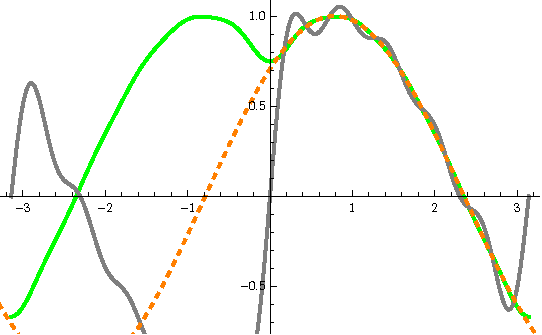
\includegraphics[width=10cm]{images/p_4a_2_33_11.pdf}
\end{center}
\subsection{Problem 16}%
\begin{enumerate}[(a)]
  \item We have
      \begin{align*}
        a_0 &= \frac{1}{2}\pi\\
        a_n &= \frac{1}{\pi n^2}\left(-1 + \left(-1\right)^n\right)\\
        b_n &= \frac{\pi}{n}\left(-1\right)^{n+1}\\
        f(x) &= \frac{\pi}{4} + \sum_{n=1}^{\infty}\frac{\pi}{n}\left(-1\right)^{n+1}\sin\left(n x\right) + \frac{1}{\pi n^2}\left(1 + \left(-1\right)^n\right)\cos\left(n x\right).
      \end{align*}
    \item Evaluating at $x=0$, we find the sine portion goes away, yielding 
      \begin{align*}
        0 &= \frac{\pi}{4}\sum_{n\text{ odd}} -\frac{2}{\pi n^2}\\
        \frac{\pi^2}{8} &= \sum_{n\text{ odd}} \frac{1}{n^2}.
      \end{align*}
      Evaluating at $x = \pi$, we get
      \begin{align*}
        \frac{3\pi^2}{8} &= \sum_{n\text{ odd}}\frac{1}{n^2}.
      \end{align*}
      The value at $x = 0$ is correct due to ringing at the jump discontinuity at $x = \pi$.
\end{enumerate}
\subsection{Problem 17}%
\begin{enumerate}[(a)]
  \item 
    \begin{align*}
      \zeta(2) &= \frac{\pi^2}{6}
    \end{align*}
  \item 
    \begin{align*}
      \frac{1}{16} &= \sum_{n=1}^{\infty}\frac{\left(-1\right)^{n+1}}{n^2}.
    \end{align*}
\end{enumerate}
\section{Chapter 34 Problems}%
\subsection{Problem 5}%
\begin{align*}
  \frac{1}{2\pi}\int_{-\pi}^{\pi} \left\vert f(x) \right\vert^2\:dx &= \braket{f}{f}\\
                                                                    &= \braket{\frac{a_0}{2}\sum_{n=1}^{\infty}a_n\cos\left(nx\right) + b_n\sin\left(nx\right)}{\frac{a_0}{2}\sum_{n=1}^{\infty}a_n\cos\left(nx\right) + b_n\sin\left(nx\right)}\\
                                                                    &= \left\vert \frac{a_0}{2} \right\vert^2 + \sum_{n=1}^{\infty}\left\vert a_n \right\vert^2 + \left\vert b_n \right\vert^2\\
                                                                    &= \braket{\sum_{n=-\infty}^{\infty}c_ne^{inx}}{\sum_{n=-\infty}^{\infty}c_ne^{inx}}\\
                                                                    &= \sum_{n=-\infty}^{\infty}\left\vert c_n \right\vert^2.
\end{align*}

\subsection{Problem 8}%
We have
\begin{align*}
  c_0 &= \frac{1}{12}\\
  c_n &= \frac{\left(-1\right)^n}{2n^2\pi^2}\\
  \frac{1}{2\pi}\int_{-\pi}^{\pi} x^4\:dx &= \frac{1}{80}\\
  \frac{1}{80} &= \frac{1}{144} + \sum_{n=1}^{\infty}\frac{1}{4n^4\pi^4}\\
  \sum_{n=1}^{\infty} \frac{1}{n^4} &= \frac{\pi^4}{90}.
\end{align*}

\end{document}
